\documentclass[tikz,border=8pt]{standalone}
\usepackage{helvet}
\renewcommand{\familydefault}{\sfdefault}
\usetikzlibrary{arrows.meta,positioning,calc}
\begin{document}
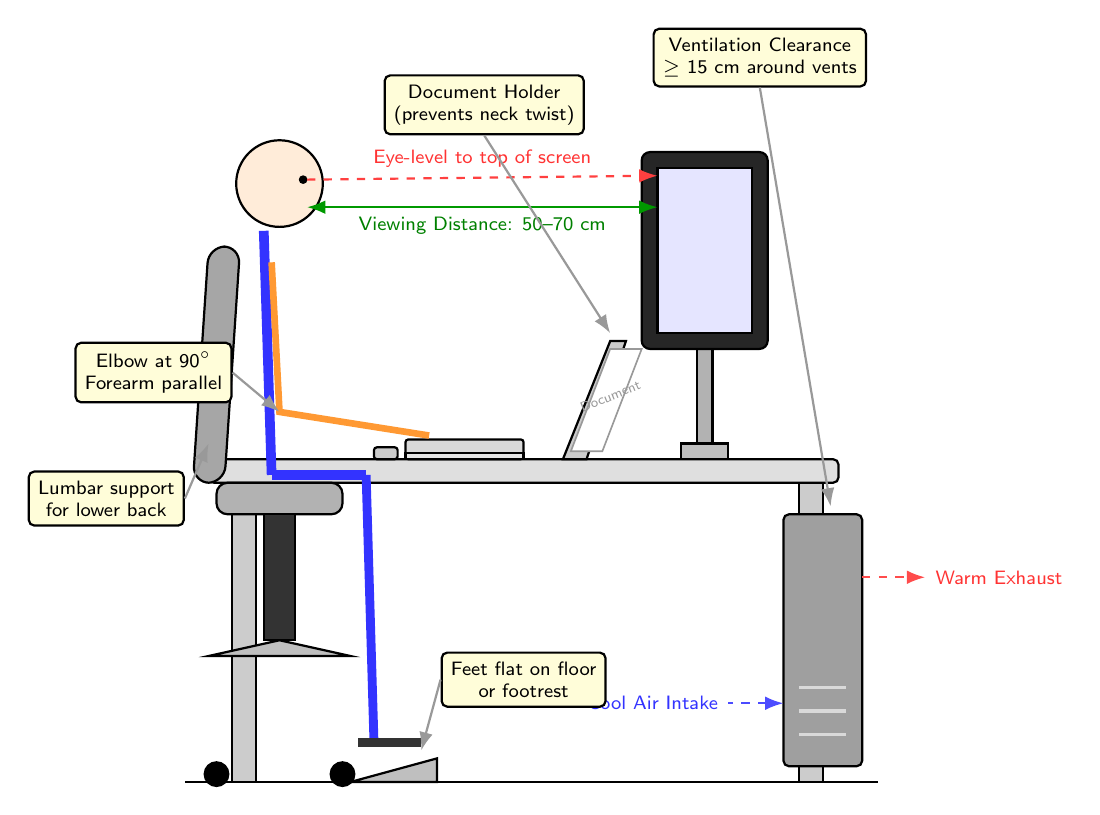
\begin{tikzpicture}[line width=0.8pt, font=\sffamily\small, >=Latex]

% ---- Desk Surface & Legs ----------------------------------------------------
\draw[fill=gray!25, draw=black, rounded corners=2pt] (1.5,4.0) rectangle (9.5,4.3);
\draw[fill=gray!40, draw=black] (1.8,0.2) rectangle (2.1,4.0);
\draw[fill=gray!40, draw=black] (9.0,0.2) rectangle (9.3,4.0);
\draw[line width=1.0pt] (1.2,0.2) -- (10.0,0.2); % floor line

% ---- Monitor & Stand --------------------------------------------------------
\draw[fill=gray!50, draw=black] (7.5,4.3) rectangle (8.1,4.5); % base
\draw[fill=gray!60, draw=black] (7.7,4.5) rectangle (7.9,5.7); % stand neck
\draw[fill=black!85, draw=black, rounded corners=3pt] (7.0,5.7) rectangle (8.6,8.2); % frame
\draw[fill=blue!10, draw=black] (7.2,5.9) rectangle (8.4,8.0); % screen

% ---- Document Holder (Paper Stand) ------------------------------------------
\draw[fill=gray!40, draw=black] (6.0,4.3) -- (6.6,5.8) -- (6.8,5.8) -- (6.3,4.3) -- cycle;
\draw[fill=white, draw=gray!80, line width=0.6pt] (6.1,4.4) -- (6.6,5.7) -- (7.0,5.7) -- (6.5,4.4) -- cycle;
\node[font=\sffamily\tiny, rotate=22, text=gray!80] at (6.6,5.1) {Document};

% ---- Ergonomic Keyboard & Mouse ---------------------------------------------
\draw[fill=gray!30, draw=black, rounded corners=1pt] (4.0,4.3) rectangle (5.5,4.55);
\draw[fill=gray!40, draw=black, rounded corners=1pt] (3.6,4.3) rectangle (3.9,4.45); % mouse
\draw[fill=gray!20, draw=black] (4.0,4.3) rectangle (5.5,4.38); % palm rest

% ---- Computer Case (Tower) with Airflow ------------------------------------
\draw[fill=gray!75, draw=black, rounded corners=2pt] (8.8,0.4) rectangle (9.8,3.6);
\foreach \y in {0.8, 1.1, 1.4} { \draw[gray!30, line width=1.2pt] (9.0,\y) -- (9.6,\y); } % vents
\draw[->, thick, red!70, dashed] (9.8,2.8) -- (10.6,2.8) node[right, font=\sffamily\scriptsize, text=red!80] {Warm Exhaust};
\draw[<-, thick, blue!70, dashed] (8.8,1.2) -- (8.1,1.2) node[left, font=\sffamily\scriptsize, text=blue!80] {Cool Air Intake};

% ---- Ergonomic Chair --------------------------------------------------------
\draw[fill=gray!60, draw=black, rounded corners=4pt] (1.6,3.6) rectangle (3.2,4.0); % seat
\draw[fill=gray!70, draw=black, rounded corners=6pt] (1.3,4.0) -- (1.5,7.0) -- (1.9,7.0) -- (1.7,4.0) -- cycle; % backrest
\draw[fill=black!80, draw=black] (2.2,2.0) rectangle (2.6,3.6); % chair stem
\draw[fill=gray!50, draw=black] (1.5,1.8) -- (3.3,1.8) -- (2.4,2.0) -- cycle; % base
\draw[fill=black] (1.6,0.3) circle (0.15); % casters
\draw[fill=black] (3.2,0.3) circle (0.15);

% ---- Human Silhouette Outline -----------------------------------------------
% Head
\draw[fill=orange!15, draw=black, line width=0.8pt] (2.4,7.8) circle (0.55);
% Eye
\draw[fill=black] (2.7,7.85) circle (0.04);
% Torso
\draw[line width=3.5pt, draw=blue!80] (2.2,7.2) -- (2.3,4.1);
% Thigh (horizontal)
\draw[line width=3.5pt, draw=blue!80] (2.3,4.1) -- (3.5,4.1);
% Lower leg (vertical)
\draw[line width=3.2pt, draw=blue!80] (3.5,4.1) -- (3.6,0.7);
% Foot on footrest
\draw[line width=3.5pt, draw=black!80] (3.4,0.7) -- (4.2,0.7);
\draw[fill=gray!50, draw=black] (3.3,0.2) -- (4.4,0.5) -- (4.4,0.2) -- cycle; % footrest

% Arm & Elbow 90 degrees
\draw[line width=2.4pt, draw=orange!80] (2.3,6.8) -- (2.4,4.9) -- (4.3,4.6);

% ---- Sightline & Viewing Distance ------------------------------------------
\draw[->, thick, dashed, red!75] (2.75,7.85) -- (7.2,7.9) node[midway, above, font=\sffamily\scriptsize, text=red!80] {Eye-level to top of screen};
\draw[<->, thick, green!60!black] (2.75,7.5) -- (7.2,7.5) node[midway, below, font=\sffamily\scriptsize, text=green!50!black] {Viewing Distance: 50--70 cm};

% ---- Callout Labels with Arrows ---------------------------------------------
\node[draw=black, fill=yellow!15, rounded corners=2pt, font=\sffamily\scriptsize, align=center] (lbl_doc) at (5.0,8.8) {Document Holder\\(prevents neck twist)};
\draw[->, gray!80, line width=0.8pt] (lbl_doc.south) -- (6.6,5.9);

\node[draw=black, fill=yellow!15, rounded corners=2pt, font=\sffamily\scriptsize, align=center] (lbl_elbow) at (0.8,5.4) {Elbow at 90$^\circ$\\Forearm parallel};
\draw[->, gray!80, line width=0.8pt] (lbl_elbow.east) -- (2.4,4.9);

\node[draw=black, fill=yellow!15, rounded corners=2pt, font=\sffamily\scriptsize, align=center] (lbl_lumbar) at (0.2,3.8) {Lumbar support\\for lower back};
\draw[->, gray!80, line width=0.8pt] (lbl_lumbar.east) -- (1.5,4.5);

\node[draw=black, fill=yellow!15, rounded corners=2pt, font=\sffamily\scriptsize, align=center] (lbl_foot) at (5.5,1.5) {Feet flat on floor\\or footrest};
\draw[->, gray!80, line width=0.8pt] (lbl_foot.west) -- (4.2,0.6);

\node[draw=black, fill=yellow!15, rounded corners=2pt, font=\sffamily\scriptsize, align=center] (lbl_vent) at (8.5,9.4) {Ventilation Clearance\\$\ge$ 15 cm around vents};
\draw[->, gray!80, line width=0.8pt] (lbl_vent.south) -- (9.4,3.7);

\end{tikzpicture}
\end{document}
